\documentclass[11pt]{report}
\usepackage{outline}
\usepackage[sfdefault]{roboto}
\usepackage{pmgraph}
\usepackage[normalem]{ulem}
\usepackage{listings}
\usepackage{geometry}
\usepackage{float}
\usepackage{longtable}
\usepackage{graphicx}
\graphicspath{{Figures/}}
\lstset{language = SQL, breaklines=true}
\title{\textbf{User Manual}}
\author{Thomas Moffat, 51337, 4042}
\setlength{\oddsidemargin}{0in}
\setlength{\evensidemargin}{0in}
\setlength{\topmargin}{0in}
\setlength{\headsep}{-.25in}
\setlength{\textwidth}{6.5in}
\setlength{\textheight}{8.5in}
%--------------------Indention
\setlength{\parindent}{1cm}

\begin{document}
%--------------------Title Page
\maketitle
\tableofcontents
\newpage 
\section{Introduction}
Welcome to Ordr, a bespoke kit ordering system! By following these few simple installation and trouble shooting steps we will ensure you get the most out of your program. This program was created for the express usage of Tilehurst Swimming Club, so should really be only used by them now shouldn't it. If you are, however, not a member of Tilehurst Swimming Club please contact the developer and sort out a version of Ordr for your own organisation. 
\section{Installation}
	To install Ordr, simply unzip the included zip file into your directory of choice. If the file names end in HTML, CSS, PHP or is kitorder2.xml, it needs to be placed on your website if it hasn't already been and needs to be linked to on the website. The rest of the files can stay where they are. Ensure that MySQL is installed on the web server, if it is not then follow the instructions found at http://dev.mysql.com/doc/refman/5.7/en/installing.html and follow the instructions for the operating system your server is running. Make sure that java is installed on your computer, from https://java.com/en/download/ and make a note of your connection settings to edit kitorder.xml with. Then once these simple steps have been followed you're ready to start using Ordr!
\section{System Description}
	\begin{figure}[H]
		\centering
		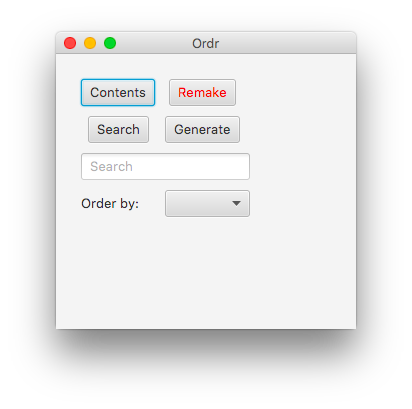
\includegraphics[scale=0.5]{MainMenu}
		\caption{The Main Menu}
		\label{mm}
	\end{figure}
	Figure \ref{mm} is the main menu. This is where you will be able to use all of the exciting features of Ordr! These include automatic Excel spreadsheet generation, search functions and more! Remember, if you click on Contents or Search and nothing happens, remember to chose the order that you want the program to show the results in.
	\begin{figure}[H]
		\centering
		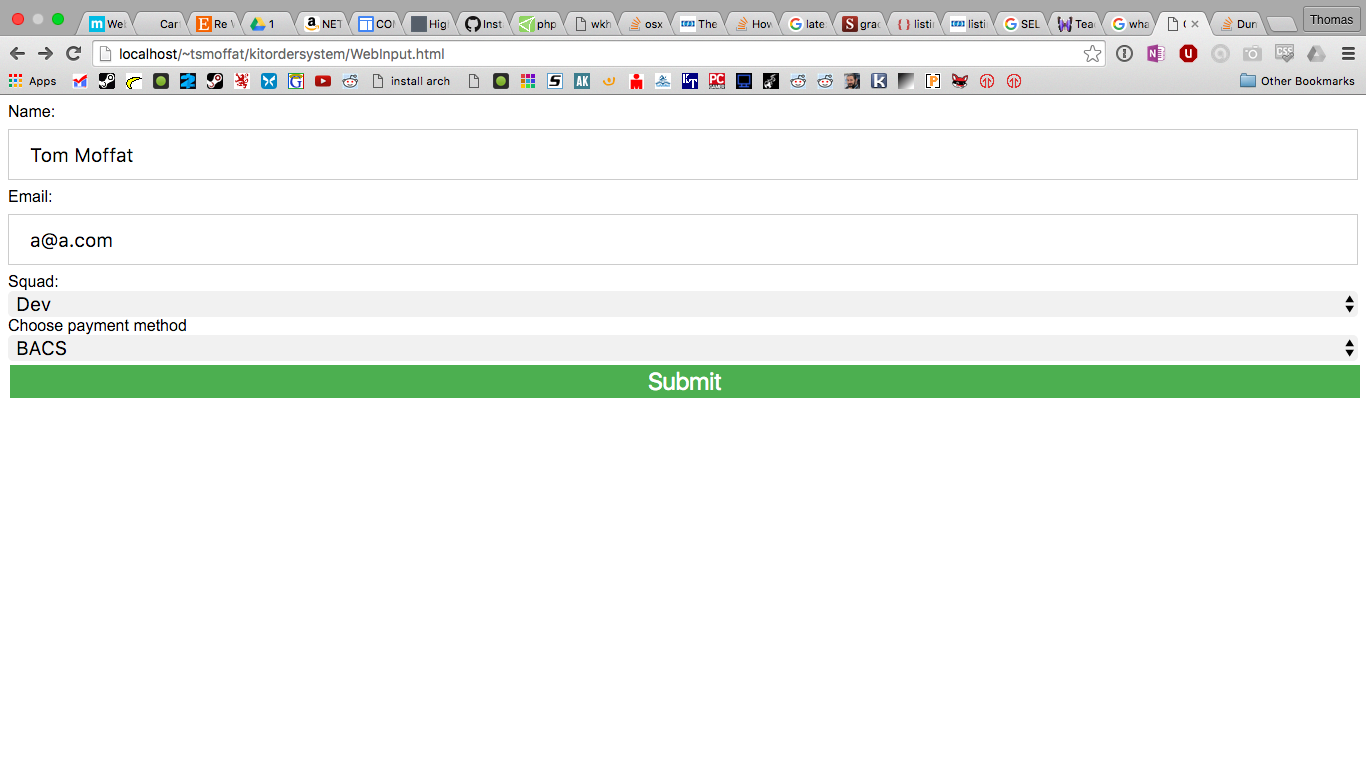
\includegraphics[width=\textwidth]{CustomerForm}
		\caption{The Customer Web Form}
		\label{cf}
	\end{figure}
	Figure \ref{cf} shows the web form that customers will see when they first open up the web order interface. This is where they can input their names, email addresses, what squad they're in and how they're going to pay for what they ordered. When they click submit, the information is loaded into the database and they are taken to...
	\begin{figure}[H]
		\centering
		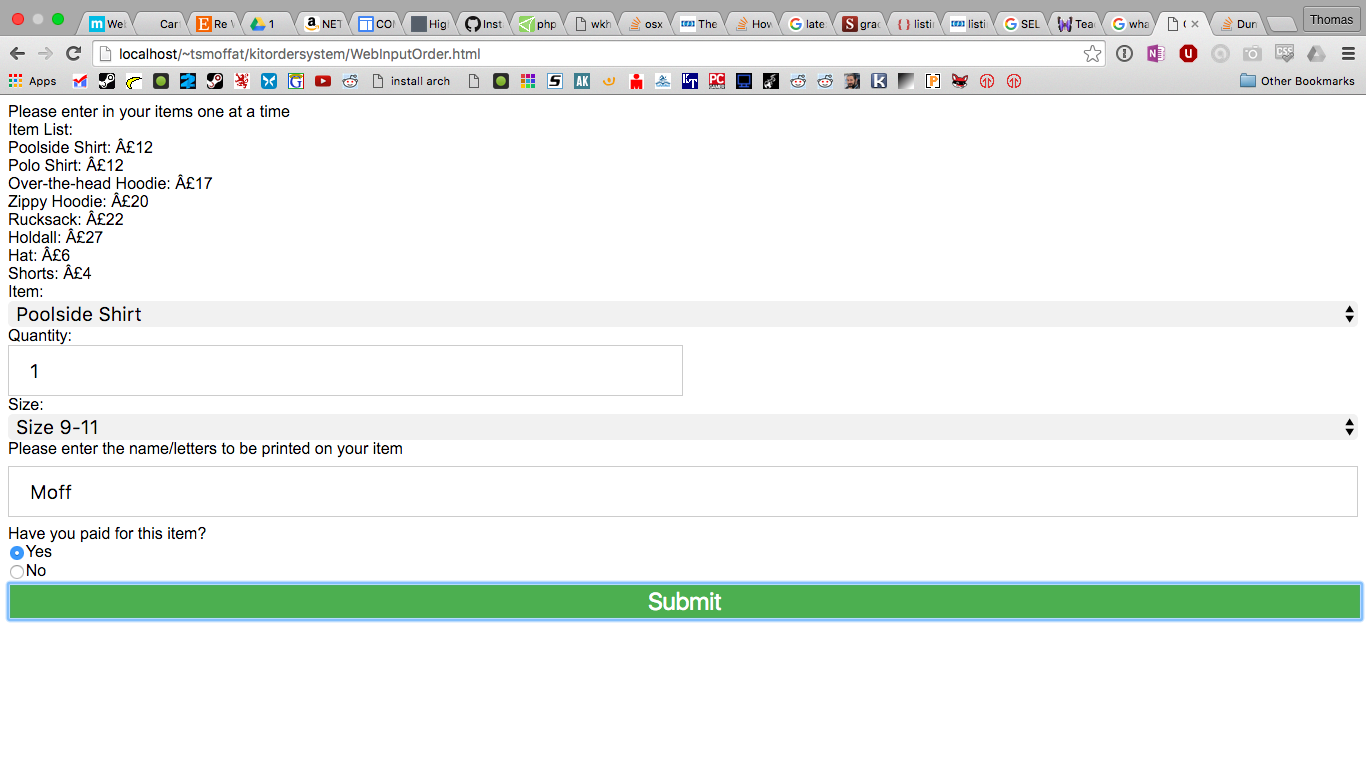
\includegraphics[width=\textwidth]{OrderForm}
		\caption{The Order Web Form}
		\label{of}
	\end{figure}
	Figure \ref{of}! This is where the customer can input the items that they actually want to purchase. When they click submit the system loads their order information into the database and the page is reloaded, ready for them to insert another item. 
	\begin{figure}[H]
		\centering
		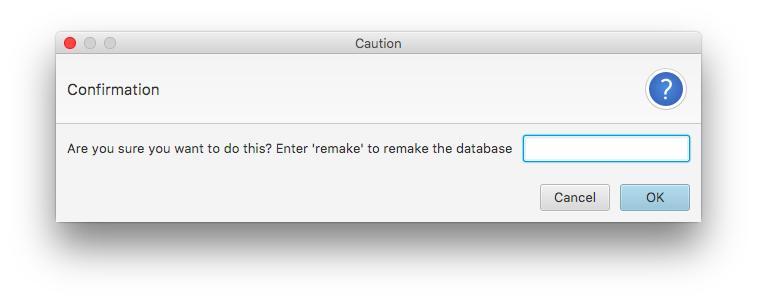
\includegraphics[scale=0.5]{ConfirmBox}
		\caption{Confirmation Box}
		\label{cb}
	\end{figure}
	This is what appears when you click the button labelled remake in red on the main menu. It's for your own safety, so you don't accidentally miss click and delete the database. If you do then don't worry! A backup has been taken of the data in the database, and is available in the directory where your copy of Ordr is located. If you clicked this and didn't mean to then just click cancel or close the box and nothing will happen.
	\begin{figure}[H]
		\centering
		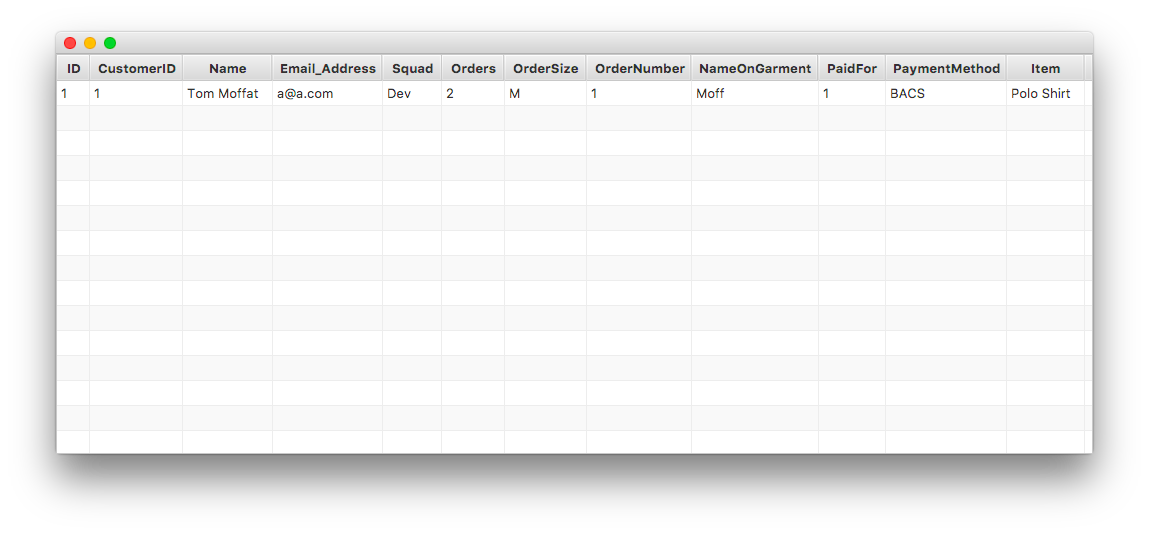
\includegraphics[width=\textwidth]{OutputTable}
		\caption{The Main Output}
		\label{ot}
	\end{figure}
	Figure \ref{ot} is what you will see when you click on Contents or Search on the main menu and you have an order set (you did remember that, didn't you?) and there is data in the database. We understand that the column headings may be slightly confusing to you, so here is a reference table to make sure you know exactly what each column means:
	\begin{table}[H]
	\caption{A handy-dandy reference table}
	\begin{tabular}{|p{0.2\linewidth}|p{0.8\linewidth}|}
		\hline
		Heading & Meaning \\
		\hline
		ID & This is the Order ID, which is automatically generated by MySQL \\
		CustomerID & This is the most recent customer ID of the customer \\
		Name & This is the customer's name \\
		Email\_Address & This shows the customers email address	\\
		Squad & This shows the squad the customer, or the customer's child, is in \\
		Orders & This shows the item ID of the item that the customer ordered \\
		OrderSize & This is the size of the item that the customer ordered \\
		OrderNumber & This is the number of items that the customer ordered. Very rarely will it be greater than 1 \\
		NameOnGarment & This is what the customer wants printed on their item \\
		PaidFor & Denotes whether the customer has paid for the item. Shows 1 for yes and 0 for no. This is sometimes referred to as a boolean value \\
		PaymentMethod & Displays how the customer has paid for the item \\
		Item & Shows the item that the customer actually ordered. This is retrieved from the Items table using the Orders column \\
		\hline
		\end{tabular}
	\end{table}
	\begin{figure}[H]
		\centering
		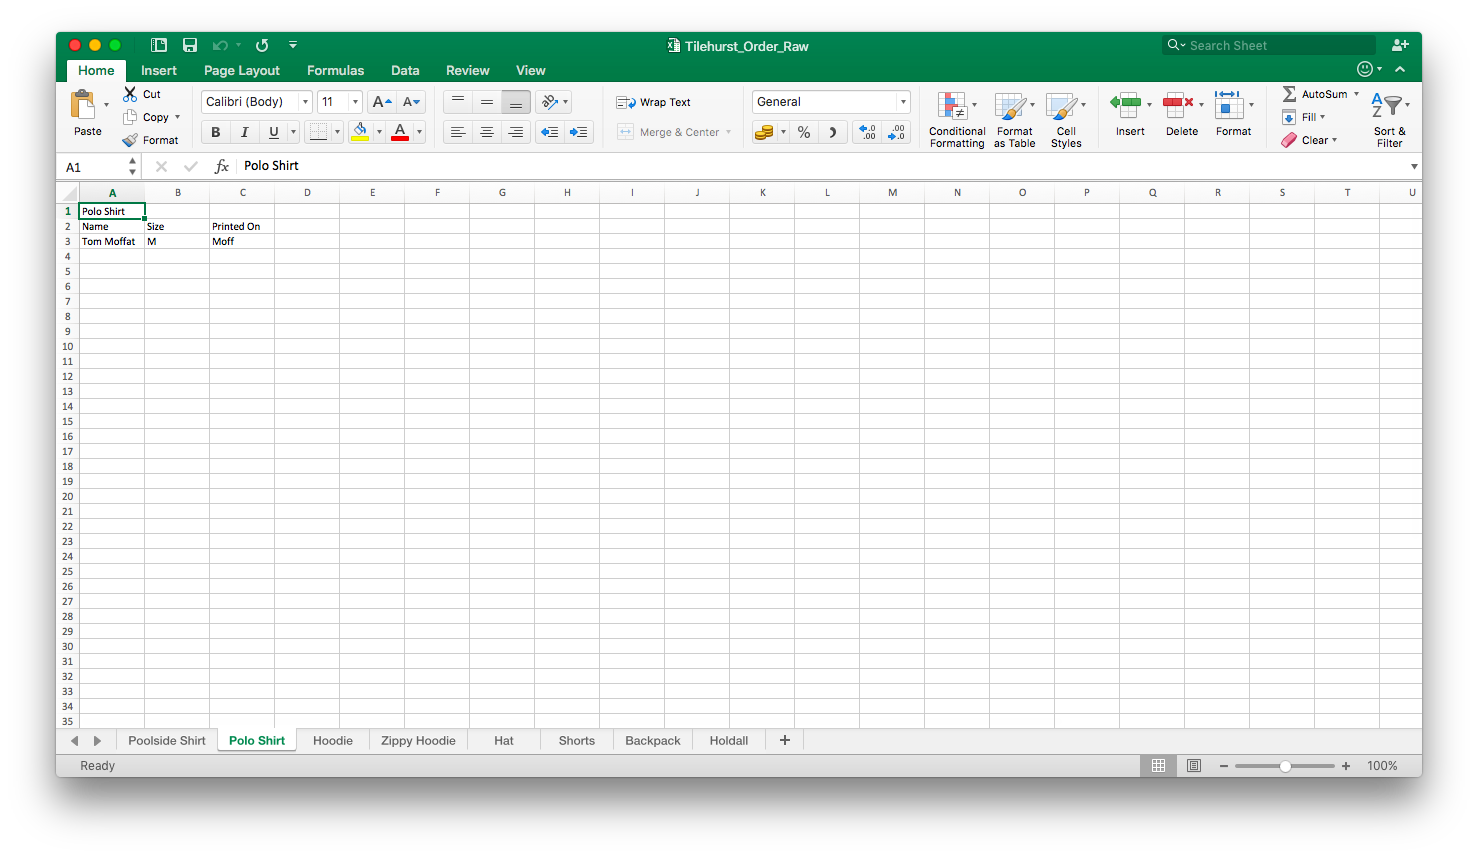
\includegraphics[width=\textwidth]{OutputExcel}
		\caption{The Output Excel Spreadsheet}
		\label{oe}
	\end{figure}
	Figure \ref{oe} shows the Excel spreadsheet that is generated when you click on the generate button on the main menu. This is meant to be used as the order form to be sent off to Cavaliers, however if you'd prefer Excel does have an option to output tables to Word. Hopefully your spreadsheet will be slightly more full than this one! To navigate between the different items just click on the tabs along the bottom.
	\begin{figure}[H]
		\centering
		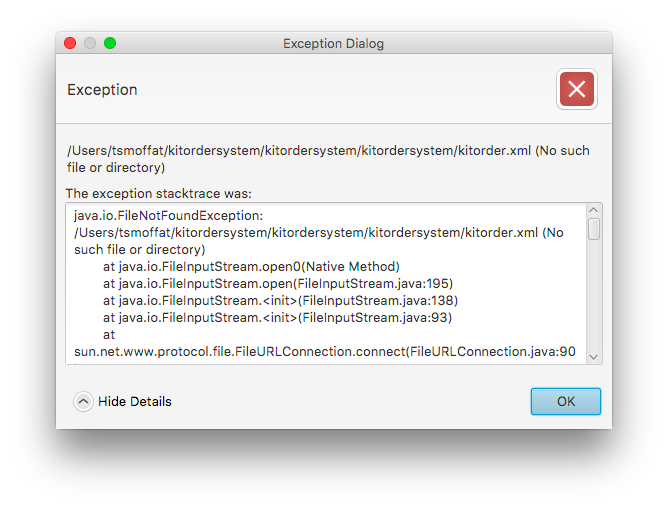
\includegraphics[width=\textwidth]{JavaUpdatedError}
		\caption{The Error Box}
		\label{jue}
	\end{figure}
	Figure \ref{jue} shows the dialog box you will get when the program encounters an error. If this happens, don't worry! Close the dialog box and try again. If it happens again, then copy the stack trace (the bit in the selectable box) and email it to the developer with the subject "Error" and a brief description of what you were doing at the time of the problem and they will get back to you as soon as is possible to help you. In the meantime, you could read what the error says and try to fix it yourself. If the error says a file is missing then try to find it, or if a message says a file already exists then move the file that already exists and try again. Small things like that then try to fix yourself but if there's anything you don't understand then email the developer.
\end{document}